\documentclass[12pt]{article}
\usepackage{multirow}
\usepackage[english]{babel}
\usepackage{multirow}
\usepackage{pdflscape}
% Set page size and margins
\usepackage[a4paper,top=2cm,bottom=2cm,left=3cm,right=3cm,marginparwidth=1.75cm]{geometry}
\usepackage{rotating}
% Useful packages
\usepackage{amsmath}
\usepackage{graphicx}
\usepackage[colorlinks=true, allcolors=blue]{hyperref}
\title{Decoding the sensation of pain from brain signals}
\author{Author: Thomas Sadler}
\date{\today}
\begin{document}
\begin{titlepage}
   \begin{center}
       \vspace*{3cm}
       \Huge
       \textbf{Decoding the sensation of pain from brain signals}
            
                   
       \vspace{1.5cm}
       \Large
       CSEE School of Computer Science and Electronic Engineering \\
       University of Essex\\
       \  24/03/2022

       \vspace{1.5cm}
       \Large
       \textbf{Author: Thomas Sadler}

       \vspace{0.5cm}
       \Large
       \textbf{Supervisor: Sebastian Halder}
            
   \end{center}

\vfill
\begin{abstract}
Due to the nature of current biology, it is hard to recognize the definition of “pain”. Pain is the most common symptom of illness that results in frequent visits to physicians for a seemingly indecisive diagnosis. By utilizing some conclusive EEG results in which a patient submerges their hands in various water temperatures, we are able to tackle one of the most consequential problems in modern medicine. This article proposes the investigation of a machine learning solution to decoding Electroencephalogram data signals and detecting pain states. The approach uses an array of standardized open-source machine learning libraries as well as niche Python frameworks to visualize, interpret, pre-process and train classification models . Although the result may not be definitive for detecting pain, it could certainly be the infrastructure on which future Computer Scientists develop their own solutions.
\newline
\newline
Keywords: EEG (Electroencephalogram), Python, MNE, MATLAB, PSD (Power Spectral Density)
\end{abstract}

\end{titlepage}
\clearpage


\tableofcontents

\clearpage


\section{Introduction}

With the technology sector making up around 7.7 percent of the UK’s economy, it seems fitting that modern artificial intelligence start to frame the way we present solutions to global problems. Machine learning is a branch of AI that uses a plethora of data and algorithms to imitate the way humans behave without having to be programmed manually. The idea behind modern classification and regression is to memorize data and present outcomes based on the previous experiments. These outcomes are what drive decision making in many corporate businesses and impact financial growth metrics. Furthermore, machine learning; whilst ever evolving, is arguably complex enough to be able to estimate biological instances that humans struggle to dictate themselves. 
As previously stated, the term “pain” tends to have a diverse range of meanings with no definitions being able to capture the entire state of the problem. Combined with either large health databases, or mere experimental study results, data scientists have the opportunity to train models to detect what humans can only infer; for example, to detect when someone is in pain. This could be done by utilizing EEG electroencephalogram data and training a classification model to recognize events deemed as a person being in a “pain” state. Although pain is counterfactual in that we cannot observe both treatments; experiments can be undertaken to simulate pain to the brain thus allowing us to evaluate the results of training a machine learning model. 
The proceeding article can be categorized into six vital sections, the first of which will be a summation of background reading in regard to both machine learning and how the data used in this project has previously been used. It will feature some referenced research paper’s and provide a brief overview of the methodologies that have been adopted, as well as the results made from their efforts. As well as previous studies, the experiment used to frame this projects data is detrimental to its success. The project background will follow with a description of the experiment conducted, and some notes on the results that were taken from its output. The project objectives will then be stated making sure to outline the focus of this article, as well as the takeaways that should be reflected by its results. As with all research paper’s that focus on machine learning; this article has limitations in regard to its scope whether the focus be on computational power or deliverable dates that need to be met without deviation. 
Arguably the most important section of this article, the technology and tools chapter will explore all the different software instruments proposed to complete the project. These range anywhere from small open-source python packages to hardware tools used to collect the data. A brief explanation into each’s inner workings will be given, as well as an insight as to how it will be used specifically in its implementation. The technology and tools will lead into a full evaluation of the proposed solution in which the author will state the project plan in the form of a Gantt chart. As well as visualizations of how the project is to be completed, the section will explore a more detailed description of the solution devised to detect pain states given our training data. Being that this project is early in its development, and no active steps have been taken to evaluate the potential success of its implementation, all the decisions made are subject to change at any point. 
The final section of this article will investigate how we plan to evaluate the validity and accuracy of our conclusions; these include: the particular machine learning metrics, how we will optimize our hyperparameters and finally how we will test our classification model

\section{Research Questions and Hypothesis}
The presence of a hypothesis in data science projects, is to predict what the author’s research will conclude. It starts by stating the problem that clearly defines the topic and producing a null and alternative hypothesis to shape the predictions of the project outcome. Typically a hypothesis determines the relationship between an independent variable (the signal data and feature matrix) and a dependent variable (our pain state) ; speculating whether on affects the other. To test a hypothesis, data scientists must first assume that there is no relationship between the two variables, in other words there will be no changes in the dependent variable due to the manipulation of our independent variable; this is referred to as our null hypothesis. An alternative hypothesis however states the opposite; that there is a distinct relationship between the variables. It also confirms that the circumstances of the experiments conclusions is not a result of randomness but support the theory being investigated. Below are the hypothesis outlined for the proposed project. 
\dots
\begin{itemize}
\item Alternative Hypothesis One: The most relevant wavelet feature will be among the 10Hz range and the location will be over the somatosensory cortex
\item Alternative Hypothesis Two: Alpha rhythm frequency will increase over the posterior regions of the scalp and decrease in the contralateral regions of the scalp when subject to pain stimulation
\item Alternative Hypothesis Three: The Riemannian classifier will outperform classic machine learning models when induced to noisy environments
\end{itemize}

\section{Project Background}
\subsection{Project Experiment}
For this project , we are evaluating the results of a controlled experiment previously conducted on multiple participants. The experiment in question involved recording the output of an EEG electroencephalogram whilst the patient engaged in 5 unique “events” all of which can be identified from \ref{fig:RawPlot}. These five events can be split further into two groups both having their own recordings that affect the EEG; these can be categorized as:
\newline
\newline
Major events
\dots
\begin{itemize}
\item Submerging hands in “warm” water
\item Submerging hands in “hot” water
\item Non-painful auditory stimulation
\end{itemize}
Resting Phase
\dots
\begin{itemize}
\item Eyes Open
\item Eyes Closed
\end{itemize}
The experiment lasted approximately 50 minutes with a controlled time of 5 minutes for each consecutive event, each of which had an affect on the EEG readings making the identification of pain states and training of a machine learning classifier significantly easier. This particular experiment was conducted on 41 different patients ensuring each patient was subject to the same events at the same times. The conditions for the hot water submersion included immersing their left hand until their wrist in a large tank of constantly circulating water, heated to approximately 45 degrees with the same conditions for the warm water submersion however with a temperature of 39 degrees instead of 45. The non-painful auditory stimulation was induced after both water submersions by playing a 5000Hz frequency through a pair of headphones. This part of the experiment was conducted not to induce pain, but to simulate a level of discomfort that correlated with the hot water submersions. Although these events are completely different, we can observe clear patterns from each event from the EEG data readings. The resting phases of each experiment involved sitting stationary with either eyes closed or eyes open; these phases occurred both before and after the three main experimental conditions. This equates to a total of 7 events for each patient Patients were asked during the recording of the experiment to rate the “unpleasantness” of each event. This allowed the authors of the experiment to take a general reading of each patient’s discomfort without considering their pain index’s thus resulting in a well-rounded dataset.

\subsection{EEG Data}
Measuring brain signals using an electroencephalogram requires the mounting of electrodes on each patient’s head. These electrodes a metal disks mounted to an elastic cap that with a combination of a special adhesive, is fitted to the patient. The EEG cap records the activity of your brain cells that communicate via electrical impulses.

\begin{figure}[tb]
\centering
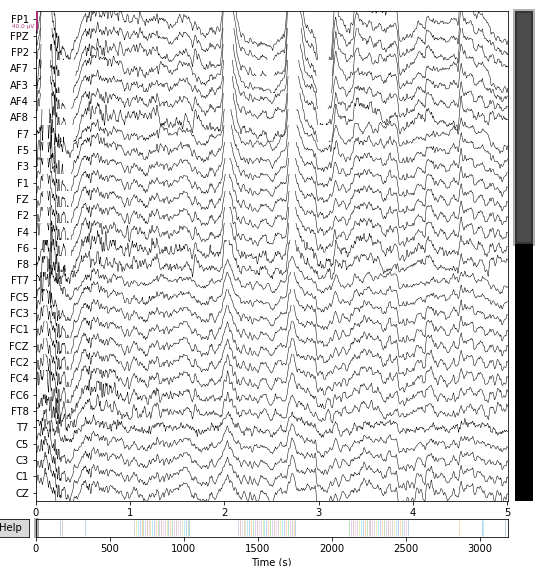
\includegraphics[width=0.95\textwidth]{RawPlot.png}
\caption{\label{fig:RawPlot}Raw data plot taken from Python measuring the EEG signals from our first patient. Each labeled line in the plot relates to a different measurement from each electrode placed on the patients scalp. Towards the bottom of the plot we can see the time scale at which our different pain states and resting phases were induced. }
\end{figure} 

The figure \ref{fig:RawPlot} below is a plot of the raw sensor traces from our first EEG experiment reading. This plot visualizes the time, frequency distribution between the readings taken from each electrode of the EEG to the brain, for example, we can see that the first label of the y-axis is referred to as FP1. Already from this simple plot we can start to evaluate some clear patterns in the data, the most notable being the initial submersion of the patients’ hands into the hot water at around 1350 seconds. From the time plot observed at the bottom of \ref{fig:RawPlot} we can easily depict the 7 different events. Our major events as previously defined can be observed as 3 blocks towards the middle of the experiment, with the 4 resting phases at the beginning and at the end in the form of single lines.

\begin{figure}[tb]
\centering
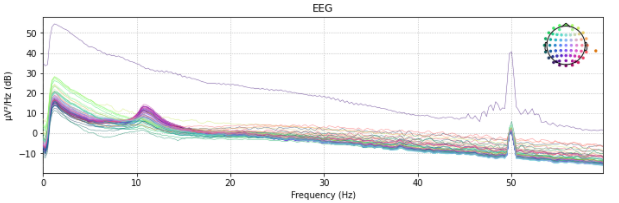
\includegraphics[width=0.95\textwidth]{PSDPlot.png}
\caption{\label{fig:PSDPlot}Power Spectral Density Plot taken from Python measuring power per Hz against frequency of the first patients EEG signal readings. Each line in the plot relates to the measurements from a particular electrode on the patients scalp. It should be noted that the line separate from the plots main tendency has been recorded as a broken electrode. The mound observed toward the 50Hz mark is as a result of the electricity grid as opposed to any brain activity and doesn't relate in any way to the patients current state.  }
\end{figure} 

As well as plotting our raw data, we can start to investigate some more in-depth visualizations including a frequency-domain power spectral density plot depicting the power per Hz vs frequency. Seeking to signify the strength variations of energy as a function of frequency \ref{fig:PSDPlot} is plotted by calling the fast Fourier transform method.

\subsection{Previous Work}
Pain state investigation is an extremely rigorously researched topic having hundreds of articles utilizing technological advancements published each year. Similar to the proposed project Guanghao Sun Et al, published an article investigating the detection of acute pain signals from human EEG data in 2020 \cite{SUN2021108964}. They were able to develop an unsupervised learning method based on multichannel human EEG recordings by using state-space model in combination with some regions of interest (ROIs) from the experiment data. From two chronic pain datasets both of which a painful stimuli were applied to the left hand of each patient, Guanghao Sun et al. collected 32-channel EEG recordings which were then subject to some simple source localization. By utilizing the MNE \cite{GramfortEtAl2013a} software package from python, the data was then pre-processed using some independent component analysis and eight regions of interest identified. From each ROI, an event-related potential was identified and the results from both data sets evaluated using standard error of mean (SEM). Although this pipeline greatly differs to the proposed project, they were successful in detecting acute pain signals given raw EEG experimental data and used a host a techniques similar to those intended from this research project i.e. the use of MNE software packages, and utilization of epoching to segment regions of interest. 
Given that this project would not be possible without the experimental data, it seems appropriate to investigate the article that produced these results, and how the data set was explored, including potential feature extraction and pre-processing methods if any. In 2019, Elia Valentini Et al assessed the “specificity of the relationship between brain alpha oscillations and tonic pain” by measuring the correlation between IAF and the patient’s individual unpleasantness score \cite{Valentini787283}. Due to the nature of this article containing a monumentally unique pipeline for assessing the relationship between alpha oscillations and tonic pain, it seems extremely unproductive to evaluate their methods, instead however we can surmise that they were indeed able to quantify the specificity of alpha oscillatory activity as an index of prolonged pain stimulation. This being said the article goes on to state that their findings were only partially conclusive with their being no difference in IAF between hot water submersion and equally unpleasant high pitch auditory feedback.
Although most articles implicate a unique method to evaluate the return of EEG experimental data and investigate the features that can be read from its contents, we can certainly be sure that EEG activity correlates of chronic pain persons that are experiencing it. MP Jensen et al. measured the EEG pattern differences between a sample of patients with a spinal cord injuries experiencing chronic pain and 28 healthy patients with no medical issues \cite{Jensen2013-ir}. The resultant data was pre-processed by removing epochs of data where unique artifacts that would skew the data including eye blinks and body movements were present. The EEG activity was then evaluated against the four frequency bandwidths (delta, theta, alpha, beta) with a series of statistical and visual exploits. The results of this article identified major pattern difference in the four frequency bands between those experiencing chronic pain, and those not; in some cases they were even able to identify which electrode sites emitted the frequency band that lead to this correlation. Their project was able to conclude that those who are experiencing pain demonstrated some recognizable EEG activity patterns meaning that the project proposed in this article is extremely warranted and should yield some interesting results that could extend that of the literature mentioned above 

\section{Project Objectives}
\subsection{Project Goals}
The goal of the proposed project is to decode the sensation of pain simulated through controlled experiments by analyzing raw electroencephalogram data and using extracted features to determine what characteristics of the data indicate a pain state. Once we are able to manually the determine which features and data patters indicate a “pain state”, we can train a machine learning classifier to detect this phenomena automatically without human intervention. Assuming these objectives are achieved there are a plethora of ways in which project can be extended and improved, an example of this would be the investigation of optimal hyper parameters when training the machine learning classifier. The achieve the listed goals, involves sequential completion of 3 main stages: pre-processing, feature extraction and classifier training / testing. Each of this components will be discussed in more detail further in the article.
\subsection{Project Limitations}
As with most machine learning projects, there exists limitation in regard to the training systems computational output power \cite{DBLP:journals/corr/abs-2007-05558}. In most cases, the systems limit positively correlates with the amount of data being used to train the model. This being said, the data being used to train the classification model in the proposed section is intending to be epoched i.e. segmented so that only the most telling parts of the data in which our major events lie are used to train the classifier. In the case that the author’s system is incapable of training the machine learning model to a degree where output accuracy is being sacrificed, the University of Essex provides options for alternative computing power (HPC High Performance Computing Cluster). Apart from the limitations mentioned above, there are no reasons for which this project should be hindered in it’s completion.

\section{Technologies and Tools}
\subsection{EEG}
An electroencephalogram (EEG) is the medical tool used to painlessly record the brain activity of those to which it has been fitted to and is the main source for data collection in the proposed project. Typically they are used to detect abnormalities in brain waves or electrical impulses at the time of simulated events and can provide data scientist the opportunity to evaluate the patterns of the brain signals at the time of occurrence. 
When an EEG is fitted, a specially trained technician will attach a number of metal discs also referred to as electrodes to the patient’s scalp using a special adhesive. In some cases however, instead of attaching each electrode directly to the patient scalp, an elastic cap will be provided with fitted electrodes that can be worn without the time-consuming connection process. Each electrode is connected with wires to an instrument that is designed to amplify the brain waves and records them on a computer system without any discomfort to the patient. Once recordings begin the patient will be instructed to sit still and avoid movements that might cause an inaccurate reading, this was not the case for the proposed project; instead of sitting still, each patient engaged in 5 trivial activities designed to prompt a unique reading from the EEG.

\begin{figure}[tb]
\centering
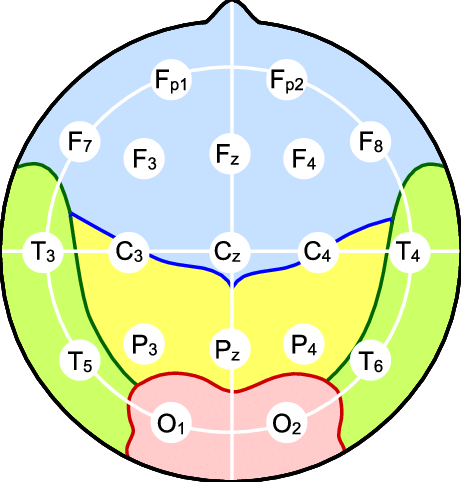
\includegraphics[width=0.5\textwidth]{ElectrodePlacementDiagram.png}
\caption{\label{fig:ECD}Labeled diagram of the 10-20 electrode placement system including the Frontal, parietal, temporal and occipital regions. This system is used to capture brain activity using an electroencephalogram.}
\end{figure} 

The method adopted by Dr Sebastian Halder Et al. was popularly used 10-20 placement \ref{fig:ECD}. The 10-20 system is a widely adopted method used to describe the locations of each scalp electrode placement. This process has been standardized over the years and is becoming more and more popular due to its ability to reproduce data readings and effectively analyse all brain signal activity. This system covers all brain regions that can be categorized as the following sections.
\dots
\begin{itemize}
\item F - Frontal
\item P - Parietal
\item T - Temporal
\item O - Occipital 
\end{itemize}
The numbering system using in combination with the lettering refers to which side of the scalp the electrode has been placed 
\dots
\begin{itemize}
\item Odd - Left Side
\item Even - Right Side
\item Z - Midline
\end{itemize}
Going back to the plot \ref{fig:RawPlot} we can see on the y-axis, each of the scalp electrode locations depicted by the 10-20 placement system.

\subsection{Python}
Python is a high-level programming language, configured to utilize object orientation and complex data structures whilst maintaining a simplistic syntax for those who are knew to coding \cite{van1995python}. It's simple to learn and massively emphasizes readability by making the visual detection of bugs extremely uncomplicated through highly developed IDE's such as Pycharm. Python offers a wide range of support modules and packages in combination with a standard library all without charge that cover almost of possible aspects of programming objectives. There is no restrictions for what Python can offer, typically the language is used to developed websites, implement new software's, visualize large bodies of data, and works to eliminate repetitive everyday tasks. 

These facts in mind, why is this programming language being proposed for this project? Aside from data segmentation and analysis, Python is widely considered one of the leading choices for machine learning projects. As of 2022, 57 percent of data scientist \cite{coursera_2021}, utilize Python for machine learning projects with statistic rising continuously as new libraries are published. Early stages of machine learning require meticulous data processing as well as data handling and transformation; Python offer all these capabilities through popular frameworks each of which is simple to learn and implement. There are hundreds of libraries that offer machine learning capabilities the most used being: Scikit-learn, Pandas, Keras, TensorFlow, Matplotlib, NLTK, Caffe and many more. These frameworks provide services that range from high-level data processing to deep learning neural training and testing. Due to the nature of the proposed project requiring data classification, Sci-kit learn will be the most useful resource, this library has been investigated in more detail further in the article.

\subsection{MNE}
MNE-Python, is a rapidly evolving open-source software package used to load, pre-process and analyze raw electroencephalogram data \cite{GramfortEtAl2013a}. Tightly integrated into Python's core, MNE enables users to create EEG data analysis pipelines by utilizing the Python programming language and creating scripts to evaluate their data. As much as MNE is designed to integrate with Python's core packages, it also works as an extension to other M/EEG analysis tools; thus making it an extremely preferable option for data scientist looking to analyze data from FIF or .set file format. MNE was first released in 2013 by Alexandre Gramfort Et al \cite{GramfortEtAl2013a} and has been undergoing scheduled maintenance constantly expanding it's capabilities and looking integrating into no collaborative programming environments.

MNE will be used predominantly for the pre-processing segment of the proposed project. Being that it works in junction with Python's core data manipulation libraries such as NumPy \cite{harris2020array} and SciPy \cite{2020SciPy-NMeth}, loading and segmenting the data is made to be seamless. Furthermore, we can take advantage of in built functions that aid us to epoch continuous data and potentially estimate evoked responses whilst utilizing capabilities offered by both core visualization libraries matplotlib \cite{Hunter:2007} and Seaborn \cite{michael_waskom_2017_883859}. This Python library alone will fulfill all the technical responsibilities of the final system up until the training of our classification model.

\subsection{Scikit-learn}
As previously discussed, Python-MNE can only take the project so far in regards to data classification; this is where Scikit-learn comes in. Scikit-learn is currently the most popular machine learning library that Python has to offer \cite{scikit-learn}. It contains a plethora of typical machine learning functionalities as well as tools for data visualization, regression models, classification models and clustering. Although SKlearn provides simplified data manipulation capabilities, it works best when in combination with a Python library specifically designed to preprocess our data; this is one of the reasons it works so successfully as an extension to MNE. There is currently no real competitor on the open market that can measure up to the machine learning potential of SKlearn apart from Tensorflow \cite{tensorflow2015-whitepaper} who specializes more with Deep learning, especially neural networks. For any system capable of utilizing the library, users will have access to the following features:
\dots
\begin{itemize}
\item Supervised Learning Algorithms (Regression models, Classification models, Support Vector Machines SVM, Decision Trees)
\item Unsupervised learning algorithms (Unsupervised neural networks, clustering, factor analysis)
\item Cross-validation (Validating the accuracy of supervised classification / regression models)
\item Benchmark datasets
\item Feature extraction 
\end{itemize}

The main features being utilized from SKlearn for the proposed project are, a supervised Classification model, feature extraction methods, and cross-validation for conclusion evaluation. One of the main objectives before the projects implementation stage is a regression model comparison in regards to our unique EEG data, Which model is equipped to handle this amount of data? Which model could be trained and tested more efficiently? Which model will yield more accurate results without compromising the projects deadlines? All of these questions need to be addressed when choosing our classification model. Feature extraction is another vital component to the implementation process; this being the reduction in features in the data set either by engineering new ones from what already exists, or using those which convey the most information about data patterns or events. Both of these processes will be investigated in more detail further in the article.

Although SKlearn isn't overly used in industry, there are still companies that utilize Python who would attest to it's simplistic yet effective use in production \cite{cournapeau}. Furthermore, many universities make this framework the scaffold on which they teach their students the basics of machine learning protocols making it the perfect choice for the proposed project.

\subsection{MATLAB}
Due to the nature of this project relying so much on EEGLAB and its encompassing software counterparts, it seems likely that the use of MATLAB maybe required at some point in the pipeline for tasks that may not be accessible by Python if any. MATLAB is another open-source software utilized by a large proportion of the world's engineers and scientists granting the ability to analyze data, develop algorithms and create applications \cite{MATLAB:2010}. Deployed since 1984, MATLAB compiles on the foundation of a matrix-based language which explains why it is one of the leading software's for most modern mathematical methods. Similar to other programming languages, it provides functionality for data analysis, data visualization and application development with the combined ability to integrate with Simulink. In most educational environments MATLAB is the go-to instructional tool for technology based mathematical courses as well as those in the engineering and computer science sector.

The potential use of MATLAB in the proposed project is based on the frequency of tasks requiring capabilities that Python-MNE cannot offer. As previously disclosed, EEGLAB is a data analytics tool similar to MNE that runs exclusively on MATLAB thus containing it's own portfolio that in some cases differs to that of it's counterpart. One of the biggest differences between MNE and EEGLAB is  it's difficulty to implement based on the users programming experience. Python is incredibly object-oriented, thus requires a limited knowledge of object-orientated concepts, furthermore Python requires the installation of several software packages and libraries considered as a prerequisite to use which may be foreign to those who consistently use MATLAB. Overall, the differences between the two software's seem to be inherently syntax based apart from the ability to create unique EEGLAB plugins via Fieldtrip programming wrappers thus making the utilization of MATLAB seemingly doubtful.

\section{Project Plan}
\subsection{Project Solution}
The solution to the proposed project can be categorized into three main stages, each of which has had it's inner details selected and evaluated using a plethora of previous publications and research justifications. Similar to most machine learning driven articles, our implementation stage will begin with the pre-processing of the raw EEG data. This "cleaning stage" will involve "epoching" the data, filtering the data both frequency and spatially based on specific parameter such as high pass and low pass frequency and finally some independent component analysis to remove artifacts and eliminate as much noise from the preliminary data as possible.

Once the data has been pre-processed, features will be extracted from the data based on their popularity from previous publications with similar objectives to our own and their probability of yielding the highest classification results given our unique dataset. It should be noted that feature extraction is by far one of the most vital areas of the project, largely influencing the efficiency and accuracy of our final model. For this reason, the features mentioned in this proposal although fixed, may be subject to variation based on future obstacles found further in the development process. 

Our final step in the solution is the classification of the input feature matrix for a resultant label prediction which hopefully should depict whether the patient is in a pain state or not. Due to the nature of our final model having a such a large influence on the project's results, it is essential that we select the model with the highest versatility towards our unique data set. For this reason the article seeks to cross examine the most popular classification models including their advantages and disadvantages as well as justify the final decision. 

In order to estimate the validity of our model, the author will begin by seeing if we can classify the distinction between our eye's open and eye's closed resting phases. The reason for this is the distinction between a pain and non pain state is extremely subtle, thus if we confirm we are able to distinguish between two more obvious states provoked by the visual stimuli, then we can be assured that our model is effective and there have been no errors in the pre-processing and feature extraction stages. The pipeline of project has been simplified in \ref{fig:Pipeline} depicting the data's journey starting from the electroencephalogram signals to a classified prediction label determining which state the patient is in. 

\begin{figure}[tb]
\centering
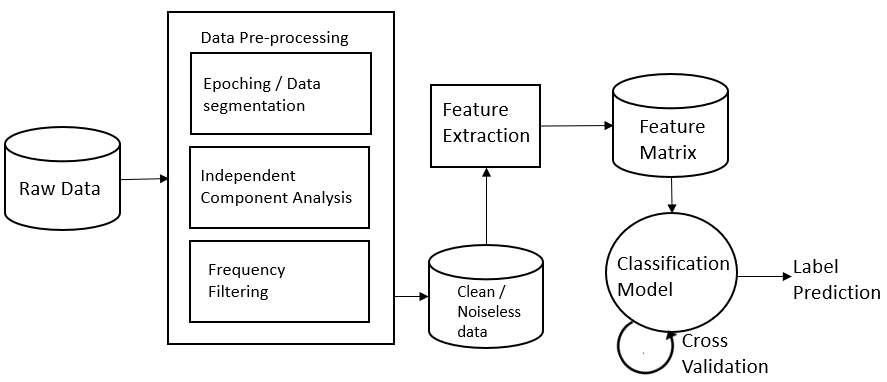
\includegraphics[width=1\textwidth]{Pipeline.png}
\caption{\label{fig:Pipeline}Pipeline of the signal data starting from raw undergoing preprocessing, feature extraction and classification resulting in a prediction label depicting the patients current state. It should be noted that any spatial filtering will take place during cross validation loop as opposed to the preprocessing stage due to it's dependence on the data's labels.}
\end{figure} 

\subsection{Pre-Processing}

Data pre-processing is defined as "the manipulation of data before it is use in order to ensure or enhance performance". Any machine learning project undertaken by modern day data scientist will have a predetermined pre-processing stage in which the data will be prepared before it use; this could be anything from removing data that isn't useful for the model training process to engineering new data from what we already know. Pre-processing in regards to signal analysis and EEG data classification typically contains generalized steps that must be seen to in order to guarantee some measure of success the first of which is referred to as "epoching".

Not to be confused with the commonly used hyper parameter "epochs" referring to the number of times a learning algorithm works through a training set, epoching is a procedure in which very specific segments of EEG signal data are extracted from a continuous source. These time windows are referred to as singular epochs, each of which depicts a unique event from the data and should be labeled based on the stimulus from which the event occurred. As shown in the magnified screen capture \ref{fig:Epoch}, we can see our 7 events of interest each of which has been highlighted with a distinct red box; these are our event phases and thus will need to be epoched from the continuous wave signal. It should be noted that the length of each epoch depends entirely on the research question under which it has been developed. This being said, for the proposed project, the epochs will not begin from the stimulus onset, rather from a baseline period in which we can clearly determine when the events have both started and finished.

\begin{figure}[tb]
\centering
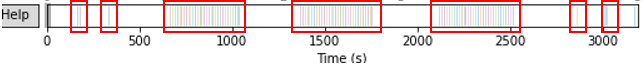
\includegraphics[width=0.8\textwidth]{Epoch.png}
\caption{\label{fig:Epoch}The experiment time scale for the first patient of which we can clearly identify our 4 resting phases, as well as our 3 major pain states. This scale modeled using Python is similar for each patient and all require epoching for extensive preprocessing}
\end{figure} 

Independent component analysis is the first pre-processing mechanism used to filter artifacts from EEG signals and reduce the presence of noise from segmented epochs. Most notably in signal processing, independent component analysis is argued to be most effective when used in combination with multi-channel signals making it optimal when classifying EEG raw data. ICA essentially works by whitening data, rotating it's matrix axis and minimizing the guassianity thus recovering independent artifacts that are statistically independent. It should be noted that Python-MNE offers services for the pre-processing methods thus rendering the cleaning and segmentation of the data effortless, furthermore the steps in this section of the article aim to be applied in the order in which they have been described. 

Another pre-processing method that needs to be applied to our dataset is filtering. There are two filtering methods to be approached, the first of which is known as frequency filtering. Essentially  frequency filtering requires that you apply both a high-pass filter and a low-pass filter to filter out frequencies that are above and below a fixed threshold. There are numerous filters that can be used to process signal data, including another filter known as a band-pass filter. This filter which can be thought of as a combination of both the low and high pass filters, is designed to pass frequencies within a predetermined range and rejects those which appear outside of it. The idea is that we are trying to reduce as much noise surrounding our events as possible and keep only the frequency at which our signal of interest operates.

The second filtering method to be applied is spatial filtering; depending on the requirements of the filter and whether knowledge of the data's labels is needed, it will take place in the cross-validation loop as opposed to the preprocessing phase. Another noise reducing process, spatial filtering works to increase the ratio of prominent signal to noise thus providing a more localized event signal to be classified. One of the most used spatial filters known as common average reference, subtracts common brain activity to the signal of interest. The idea is that we are trying to remove averaged brain activity that can be characterized as not being one of our seven induced events. Another common filter often referred to as common spatial patterns (CSP) once again works to maximize the discriminability between two classes of signal thus isolating our event later to be classified. Often regarded an extension of common spatial patterns is SPoc. SPoC, source power comodulation extracts spatial filters and patterns using continuous variables in the decomposition process. It's typically used for the extraction of motor and audio patterns using sound envelope however has been experimented thoroughly for pain classification. Although both frequency and spatial filters can be extremely useful for cleaning our data, there have many publications stating that unnecessary signal filtering can cause EEG signal shape distortion thus we must evaluate our accuracy on a continuous basis whilst applying significant filtering techniques.


\subsection{Feature Extraction}

Feature extraction is argued amongst data scientists to be one of the most vital processes in electroencephalogram signal classification. It refers to the transformation of raw data into numerical features that can be evaluated and used to train a classification model with the goal of predicting our patient states and ultimately detect pain. Numerous articles published over the years can attest to the improvement in results in machine learning utilizing newly engineered features as opposed to raw data. Extracting features from raw data can be either done manually or automatically but typically extracting features that have proven to be useful for unique objectives yields more accurate predictions. Although neural network layers are working to replace feature extraction, it remains the most effective pre-processing mechanism for time-series applications and most notable in our case, signal classification. Raw data tends to have a large percentage of information redundancy, especially in regards to the brain of which their is so much data being expelled; for this reason feature extraction works to identify the most insightful signal characteristics and classify based on those alone.

Choosing the features for the proposed project is an extremely open ended process. There are currently hundreds of different features that demonstrate discriminatory characteristics when pain is induced, only a few of which will yield the results accurate enough to determine which pain state our patient is in. This section of the proposal has been designed to offer a multitude of feature comparisons. Each feature will be explained in conjunction with it's advantages and disadvantages as well as it's usefulness weighting for our unique objectives determined. We will conclude with the final features / feature extraction methods chosen for the project. 

One of the most popular feature extraction methods used in combination with pain detection is by far wavelet transformation. Wavelet transformation essentially translates the time-amplitude representation of a signal to the time-frequency domain which is then wrapped as a set of wavelet coefficients. Once one has these wavelet coefficients, you can manipulate them to achieve a variety of signal processing effects, a lot of which have identifiable characteristics when measured by a patient in a pain state. Over the last ten years, there have been numerous studies exercising wavelet transformation to classify pain states. In 2017, Rami Alazrai Et al. published an article proposing a recognition system that used wavelet transform to identify tonic cold pain \cite{Alazrai2017EEGbasedTC}. They essentially constructed a two-layer classification framework, comprised of a number of non-linear HOS-based features, including: Skewness, Kurtosis. They were also successful in engineering auto-regressive coefficient-based features including both entropy and energy. The methodology adopted in this project correlates to this article in many aspects, most notably, differentiating between pain states and resting phases. Post implementation, the Rami Alazrai Et al. were able to conclude successful results from the two layer classification model, this includes 93.86 and 90.18 percent accuracy from the two layers respectively. Another article which demonstrates the usefulness of wavelet transform in regards to pain classification was published by Leontios J. Hadjileontiadis Et al in 2019 \cite{7055273}. By experimenting with high order spectral features as opposed to non-linear features, the company was able to produce results of a similar impressiveness as Rami Alazrai Et al. Alongside being experimentally proven to be effective, wavelet transform also offers a number of characteristics that benefit our unique data set; mainly it's interpretation of non-stationary signals. Typically wavelet transform produces a three dimensional feature space consisting of time, frequency and location. This being said the time resolution is not equivalent for all frequencies, depending on the level of frequency, it's width can vary. 

Another popular feature extraction method commonly used with EEG data analysis is fast Fourier transform. Fast Fourier transform. by mathematical means, uses power spectral density (PSD) estimation to represent EEG sample signals. Although widely used in industry there are a plethora of disadvantages that make FFT unsuitable for the proposed project, most notably it's inability to effectively interpret non-stationary data signals such as EEG. Essentially when fast Fourier performs signal decomposition, the wave frequency is split into two different components both of which can be misleading when compared to the original wave, this can cause results to skew and ultimately affect the performance of the classification model. Noise sensitivity and the presence of artifacts in signal data is another major obstacle with which our feature extraction methods need to be able to contend with; fast Fourier transform suffers heavily from noise sensitivity thus cementing it's estrangement in the project.

Eigenvector-based feature extraction, dissimilar to Wavelet and FFT, is a dimensionality reduction technique that works to extract features by implementing certain functional mapping; it does this by keeping as much data as possible from the raw data set when performing the transformation. Eigenvector feature extractions greatest advantage is it's ability to thrive when working with noise-buried data. Being that the project proposes a rigorous pre-processing phase in which a large majority of the artifacts and signal noise will be removed, it seems redundant for the technique to be used.

While these conventional feature extraction methods consider the regions of the brain independently, connectivity measures the connection between brain regions, and measures the dependency of brain activity. Although there have been no recent studies demonstrating the effectiveness of brain connectivity in relation to pain detection, there have been numerous studies recognizing it's success in classifying emotional states in patients \cite{MOON202096}. Seong-Eun Moon et al 

Although feature transformation methods can provide a general depiction of how features extracted via those means will perform, there are numerous studies that justify specific feature performances when detecting pain states in particular \cite{10.1093/cercor/bhaa124}. Typically, alpha waves oscillate between roughly 8 and 14 Hz with patients at upper end demonstrating much more resilience when inflicted with pain and more susceptible toward the lower end. In 2020, Andrew J Furman conducted an experiment in which the objective was to measure 61 healthy patients alpha waves, before and whilst being subject to a painful stimulant. The results from the experiment yielded an extremely promising conclusion with a large percentage of the patients exhibiting noticeable susceptibility and resilience patterns. It should be noted that the results of this experiment were confirmed by a secondary assessment conducted approximately 8 week after the first. 

In order to grant a more surmised view on feature extraction techniques and their effectiveness in relation to pain, a table has been created to depict the advantages and disadvantages of each. It should be noted that although no mention of Time frequency analysis and auto regressive features has been made in this proposal, it has been included in the table to present an element of completeness in regards to feature extraction methods.

\begin{center}
\begin{tabular}{ |c|c|c|c| } 
\hline
Feature Extraction & Advantages & Disadvantages\\
\hline
\multirow{4}{5em}{Wavelet Transform}
& - Literature Supported & - Commonly used \\ 
& - Suited to non-stationary signals  & \\ 
& - Detects sudden signal changes &  \\ 
& - Accurately interprets irregular patterns & \\
\hline
\multirow{5}{5em}{Fast Fourier Transform}
&- Faster than other Extraction methods  & -  More suited \\ 
&- Can be accurate if utilized properly & to stationary\\ 
&  & Signals \\ 
&  & - Suffers from \\ 
&  & Noise Sensitivity\\ 
\hline
\multirow{3}{4em}{Eigenvector}
& - Handles noisy data very well  & - No previous\\ 
& & publications \\ 
& &  \\ 
\hline
\multirow{4}{5em}{Autoregressive}
& - Performs well on short data segments & - Can be difficult \\ 
& - Yields an impressive frequency resolution & to work with \\ 
&  & - Largely affected \\
&  & by data biases \\
\hline
\multirow{5}{5em}{Time frequency analysis}
& - Great for continuous data segments & - More suited \\ 
& - Very proficient with clean data  & to stationary \\ 
&  & signals \\ 
&  & - Requires vigorous \\ 
& & Preprocessing \\
\hline
\end{tabular}
\end{center}

We can clearly observe that the advantage to disadvantage ratio of wavelet transform outweighs that of the other feature extraction methods making it the best choice for the proposed project. Although not adopting other mechanism will restrict the project in regards to variability, the project means to investigate different classification models as well as spatial filters to ensure a complete oversight of the topic with some varied hyper parameters that will make for some interesting result comparison. 

\subsection{Data Classification}

Once the data has been cleaned, all artifacts removed, and features extracted to obtain our feature matrix; a selection of classification models will need to be trained in order to process our data and predict our labels. Note that multiple models will be used to evaluate the effectiveness of our features from multiple standpoints.The idea of a classification model is to draw a conclusion from a set of input values and make a prediction for the label target; the input values in our case will be our feature matrix, and our labels will either be: whether the patient is in a pain state, or the pain index they are feeling. Similar to finding a feature extraction method, the determining of the project's classification models requires a comparative approach with each model having optimally obtained significant literature support.

Support vector machine classifiers are one of the most common and well performing models used in signal classification. They work by taking each label, and determining a hyper plane which best separates each of them. This can also be referred to as a decision boundary; anything that lies outside of a particular labels decision boundary, is considered an entirely different label. In 2019, Alazrai Rami et al. were able to demonstrate the use of a support vector machine classifier to detect tonic pain in patients given features from their respective EEG signal readings. They constructed a binary classifier used to classify patients signal readings into both pain and non-pain states; extremely similar to that of this proposal. Another useful publication authored by Gaurav Misra et al. investigated the comparison between logistic regression models and support vector machines and found SVMs to yield a far superior accuracy when used in combination with either the linear kernel or the Gaussian kernel \cite{Misra2017-xt}. Typically support vector machines perform  well when faced with highly dimensional feature sets, furthermore the model exercises it's versatility by offering multi kernel functionality which can be applied to buffer the accuracy levels of any output. With little to no major disadvantages to speak of, this classifier is an one of the primary candidates for the project, it has been continuously backed in cases of machine learning literature as well as offering characteristics that are highly preferable in regards to our unique data.

Another classifier implored by Gaurav Misra et al. was the logistic regression model. Different to the support vector machine, logistic regression is a classification technique that utilizes a more statistical approach. Typically when using a logistic regressor, there tends to be one or more independent variables that determine an outcome; these in our case are the features extracted from the EEG signal data. The intention is that the mechanism attempts to find a best fitting model that can adequately depict the relationship between both these features, and the dependent variable. Similar to other classifiers, the logistic regressor can adapt to either a binomial or multinomial model, dependent on how many different labels we are trying to predict; this could be extremely useful for those attempting to classify both pain, and the index of the pain being felt. This being said the model is tends to be more popular with binary outputs. Although the characteristics for a logistic regression classifier align with the requirements of our data, Gaurav Mistra et al. were able to prove the model to be far inferior to the support vector machine with the latter yielding a significantly higher prediction accuracy. These facts in mind it would be counter intuitive to retest the model against what we already know to be true through previous literature.

Although rising in popularity of the last few years, the Riemannian classifier is still a sparsely used classification model amongst data scientists. Riemmanian classification as oppose to conventional classification does not estimate spatial filters or select features, instead it maps data directly onto a geometrical space in combination with a suitable metric. The space onto which the data is mapped can be used to classify the data by local and linear approximation. Although there hasn't been any obvious publications made that evaluate the effectiveness of Riemannian models for pain classification, there is a plethora of literature regarding it's use in general classification studies in the EEG signal space. The processing procedures of Riemannian approaches are typically simpler and involve fewer stages than other classification models, furthermore F. Lotte et al argues that the Riemmannian classifier "applies equally well to all BCI paradigms" whether it be mental imagery, ERP, SSVEP or potentially pain classification \cite{Lotte2018-ex}. As well as being versatile in the signal classification space, the model is also parameter-free meaning that it does not require any tuning to maximize it's accuracy thus lightening the workload during the cross-validation phase of the project without sacrificing the quality of our output. Baring in mind the plethora of benefits Riemannian classification boasts as well as it's unexplored potential, it would be a wasted opportunity not to test it's effectiveness in regard to pain classification.

Similar to support vector machines, there is a vast literature investigating the effectiveness of random forests to classify pain. Another supervised machine learning method, random forests are essentially a collection of decision trees all consisting of three constituent parts; Nodes, which tests for the output of a particular attribute, edges, which depict the outcome of a test and connect to the next leaf, and finally leaves also referred to as terminal nodes that seemingly predict the outcome of that decision tree. Random forests tend to be infinitely more accurate then a single decision trees as well as producing significantly accurate results without the prerequisite of extensive hyper parameter tuning. In 2017, Vishal Vikayakumar et al. were able to classify tonic thermal pain across 20 patients from their EEG readings using random forest models \cite{Lotte2018-ex}. They used this model to predict five different pain indexes using time-frequency wavelet representations of independent components and the relative importance of each frequency band resulting in a mean accuracy of 89.45 percent. This is argued in the article to be one of the "highest accuracies among existing state of the art quantification algorithms for EEG" making it an extremely preferable choice for the project. 

\subsection{Methodology}
The methodology chosen to manage this project is that of the agile methodology. Agile software development refers to an iterative process that involves constant supervisor communication with requirements and solutions that evolve through consistent collaboration. In particular, this project will adapt the Kanban technique which is an effective subset of agile. Kanban is a work management system designed to help you visualize your work, minimize work in progress states and maximize project efficiency. Although Kanban is argued to be most beneficial when used in conjunction with large teams, It can be extremely effective at helping sole workers organize their software development stages, maximize time constraints, and reach goals through with an effective work life balance. Most kanban systems come in the form of a "Kanban Board" on which you can define your four main columns: Backlog, Selected for development, In progress, and Done. These columns are used to store issues and tasks delegated during the design stage of the software development process, with more issues being added as the project unfolds. One of them most beneficial components of the agile methodology is being able to continuously retrace to previous stages and make changes based on future or current progress, furthermore with an iterative approach, requirements and implementation strategies can be elicited at any stage of cycle allowing decision to be made based on current conditions rather than predictions on how the system will look several weeks in advance.

There are two major tools that will surely be complicit to the projects success. The first is Jira project management software. Jira is a software that offers agile project management capabilities including that of Kanban boards. Using Jira, weekly issues and sub tasks will be set to the boards with a time constraint suitable for the difficulty of the task itself. It will be ensured that these issues are conveyed to the project Supervisor with sufficient task segmentation to break down the larger tasks not designed to be completed within a weeks time period. Upon the projects completion, a compilation of the Kanban burn down charts will be made surmising the weekly progress during each phase of the software development cycle and detailing whether every deadline was kept to. Any tasks that have been misjudged in time required to complete, will be re-entered into the boards backlog and seen to at the nearest date at which the author has no other engagements pertaining to the projects progress.

The second project management tool is the popular open-source software GitHub. GitHub is a version control platform allowing users to access work from any web enabled device in the world. GitHub requires a plethora of version control skills including management of branches and repositories as well as knowing how and when to commit push and pull requests. GitHub will be used mostly to store, develop and maintain any files pertaining to the project that require imminent storage and multi-geographical access. 
\subsection{Gantt Chart}

\begin{landscape}
\begin{figure}[tb]
\centering
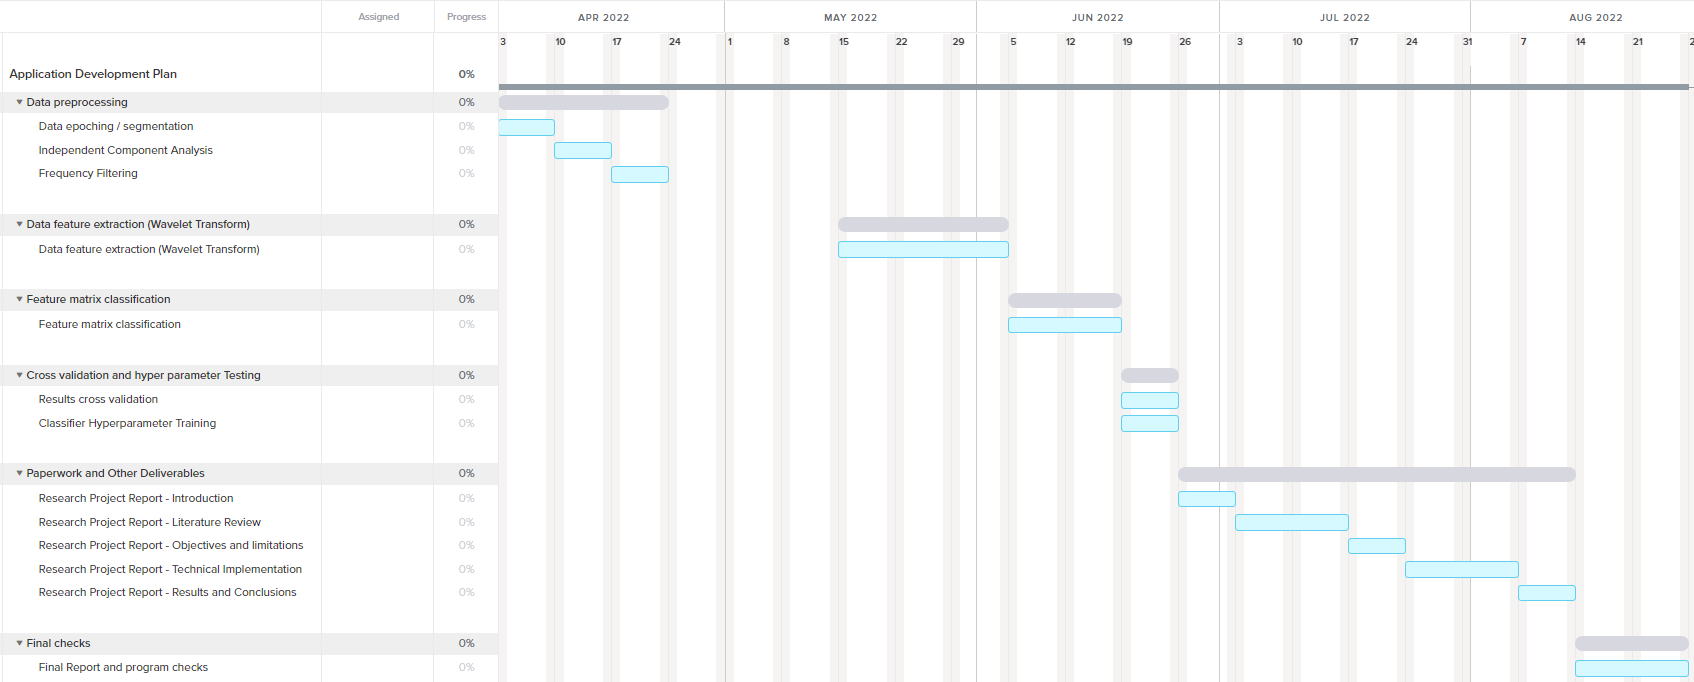
\includegraphics[width=1.7\textwidth]{Gantt.png}
\caption{\label{fig:Gantt} Gantt chart depicting the timeline under which the project will be carried out to completion. The chart has has 6 phases each of which has been given a strict deadline. This scale has been plot using weeks as opposed to days and doesn't account for weekends.}
\end{figure}
\end{landscape}

This gantt chart \ref{fig:Gantt} was designed to to provide some insight into the timeline of which each stage of the project will be completed. The timeline has been broken down into the three main stages of implementation that have already been mentioned, as well as time given for cross validation, deliverables / paperwork, and final checks towards the end of the University term. It should be noted that although the development process has already been planned, improvisations may have to be made for setbacks in progress or objectives that are hit before their deadlines; furthermore as with all machine learning proposals, there is bound to be some unforeseen tasks that will need to be addressed as an when they appear. The breakdown of each phase is as follows:
\dots
\begin{itemize}
\item Data Processing: Epoching (7 Days), Independent Component Analysis (7 Days), Frequency Filtering (7 Days)
\item Feature Extraction: Approximately 3 weeks
\item Feature matrix classification: Approximately 2 weeks
\item Cross validation: Hyperparameter optimization (3.5 Days), Result cross validation (3.5 Days)
\item Paperwork: Introduction(7 Days), Literature Review (14  Days), Objectives and Limitations (7 Days), Technical Implementation(14 Days), Conclusion(7 Days)
\item Final checks: Approximately 2 weeks 
\end{itemize}

\section{Evalution}
\subsection{Hyperparameter Testing}

Often in machine learning, a user will not immediately know the optimal architecture for any one classification model. Machines have been developed since to automatically explore the parameters of which the model relies on to perform at an optimal level; these parameters are referred to as hyperparameters. Unfortunately there is no way to know which hyperparameters are optimal for your model without some kind of experimentation; for example if our training model is a random forest classifier comprised of a collection of decision tress, how many trees should I use?, furthermore at which depth should I set the limit for each of our trees? Determining these values is done using various hyperparameter tuning methods. 

Possibly the most common method used by data scientists is Grid search. Grid search can be thought of as an exhaustive approach; manually defining the parameters at which to train the model and identifying that which yielded the highest score. Another common hyperparameter tuning method is random search. As opposed to grid search, random search uses a statistical scale around which values for the model are randomly sampled. Both of these methods will be tested against our three models with the results being evaluated through a comparative means.

\subsection{Cross validation}

Cross validation, the final stage in the project is a statistical method that works to estimate accuracy of our trained classification models. Often referred to as k-fold cross validation, the process involves shuffling the data and splitting the data into specified k groups. For as many loops as k i s equal , each group is tested against a model that has been trained using the other unique groups, the evaluation score is retained and the model discarded. The overall performance of the model is summarized using a sample of the evaluation scores. This essentially means that each unique group would have been tested against the model once, and used to train the model k-1 times. It should be noted that any hyperparameter tuning or preprocessing extensions such as spatial filtering should take place inside of the loop as opposed to outside so as to avoid in any data leakage. Often to weigh the effectiveness of different classification models, mean evaluation scores are compared with the highest mean depicting the best performing model; this process will be a similar process in the proposed project. 

Although this article has frequently outlined the steps required to segment and remove artifacts from the data inside the preprocessing phase, there are some processes that will alternatively take place within the cross validation loop. This is completely dependent on whether the process requires knowledge of the whole signal recording, for example, training a common spatial filter on the entire data set including the the data's label must be done inside the validation loop, similar to spatial filtering both frequency filtering and independent component analysis require knowledge of the labels; this being applying these mechanism's inside the pre-processing phase is more tolerated so as to establish significant baseline for the project. 

\bibliographystyle{abbrv}
\bibliography{Citations}


\end{document}




